\chapter{Outlining for Segmentation}%
\label{cha:contribution_outlining}

\minitoc%

\newpage%

Interactive segmentation consists in building a pixel-wise partition
of an image, into foreground and background regions,
with the help of user inputs.
Most state-of-the-art algorithms use scribble-based interactions
to build foreground and background models,
and very few of these work focus on the usability of
the scribbling interaction.
In this chapter, we study a very intuitive interaction
to non-expert users on touch devices, named outlining.
We present an algorithm, built upon the existing GrabCut algorithm,
which infers both foreground and background models from a single outline.
We conducted a user study on 20 participants
to demonstrate the usability of this interaction,
and its performance for the task of interactive segmentation.


\section{Introduction}


The number of pictures that are captured,
stored and shared online is growing everyday.
In march 2017, Facebook reported that 300 million pictures
were uploaded each day on their website.
These pictures are increasingly used by companies
and individual users, enabling new applications
trying to improve everyday life.
Object segmentation serves as an important step
toward automatic image understanding which is key
to those smart applications.


Object segmentation in an image remains a challenging task.
This process of assigning a label to each pixel is very sensitive
to the classical difficulties encountered in computer vision
such as lighting conditions or occlusions.
Recent advances in deep learning have enabled researchers to obtain
state-of-the-art results~\cite{long2015fully} by training
on the PASCAL segmentation dataset~\cite{everingham2010pascal}.
Some other techniques learn to infer a pixel-wise segmentation
from weak annotations, i.e.\ bounding boxes around
objects~\cite{papandreou2015weakly}.
These methods are very promising but need huge amount of human labeled
samples in order to train deep neural networks.
Recent approaches have tried to overcome this issue,
introducing active learning to train deep neural networks
using a limited amount of selected samples~\cite{liu2017active}
on the problem of image classification, but none of these methods
have yet been applied on semantic segmentation.
% \alert{This statement was true in 2017, to be verified.}


Since fully automatic segmentation is still in many cases
out of algorithms' reach, researchers have introduced
the concept of interactive segmentation.
This problem has often been approached with a task-driven point of view:
what type of interaction may bring the necessary information
to significantly help an algorithm achieve an acceptable segmentation?
The users providing the interactions are often supposed
to have a fair understanding of what segmentation is.
This assumption is problematic, especially when putting
into perspective the extraordinary amount of images to be annotated.
That is why our target audience is composed
of non-expert users who are not knowledgeable
about image processing and segmentation.
As a consequence, most of the existing work are not suitable to our problem.
They rely on foreground and background scribbles
requiring high cognitive load from the users.


\begin{figure}[h]
\centering
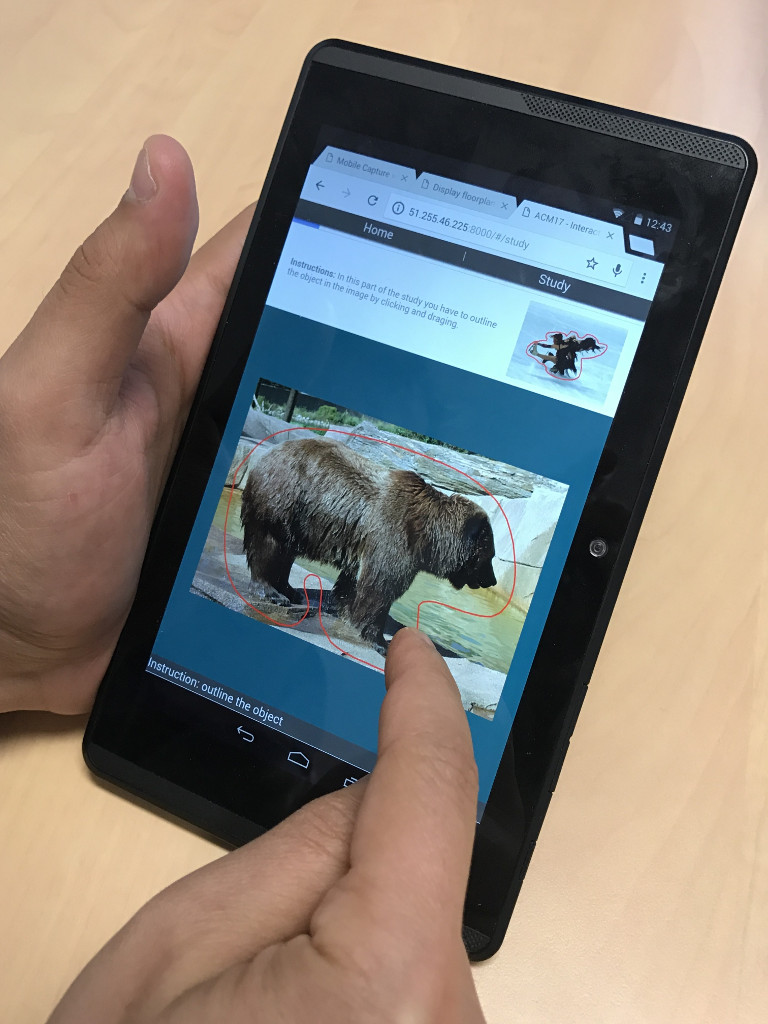
\includegraphics[width=0.4\columnwidth]{assets/img/photo_tablet.jpg}
\hfill
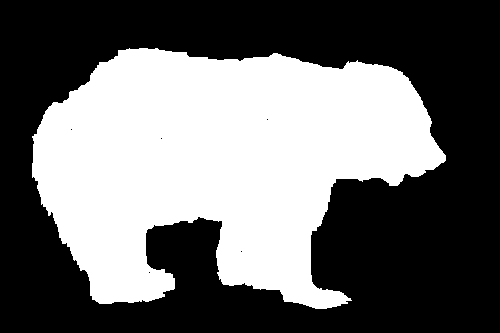
\includegraphics[width=0.55\columnwidth]{assets/img/bear_02_mask.png}
\caption{A user outlining an object on a touch device,
and the resulting segmentation mask obtained with our method.}%
\label{fig:bigpicture}
\end{figure}


Instead, we propose to use an intuitive interaction,
outlining (Figure~\ref{fig:bigpicture}),
that can be performed quickly and lead to good segmentation results
while keeping users from entering a process
of iterative segmentation refinement.
This outlining interaction is particularly well suited
for touch devices, which is appropriate considering the growing
usage of tablets and smartphones compared to computers.
All these properties make the outlining interaction very interesting
for crowdsourcing segmentation annotations on thousands of images,
with non-expert users.


We present two main contributions in this work:
first, a modification of the GrabCut algorithm
that takes as input an outlining interaction, instead of a bounding box.
We take advantage of the free-form shape drawn by the users
to extract information about foreground
(using the Blum Medial Axis computation)
from a background annotation (the outline).
The second contribution of this work is the usability comparison
of various interactions used in interactive segmentation.
We argue that the outline offers the advantage of being a quick,
easy-to-understand and usable interaction while providing
a high amount of supervision to obtain a good segmentation.


The rest of the chapter is organized as follows. Since we have already
extensively described the state-of-the-art in the previous chapter,
we first introduce the outlining interaction along with our method
to compute segmentation masks in Section~\ref{sec:method}.
We then present in Section~\ref{sec:experiment} our experiments and the results
showing that our simple interaction leads to segmentations of good quality.






%\subsection{Interactive segmentation for non-expert users}


%Although many work have studied how to incorporate human interactions
%into segmentation algorithms, there are only very few authors
%who studied interactive segmentation with a special focus
%on the interaction matter.
%In particular, the distinction between expert and non-expert users
%has rarely been made when studying
%the performance of interactive segmentation algorithms.
%Considering the tremendous number of ground truth masks needed
%to train deep learning algorithms to segment images,
%the human annotations necessarily have to be provided by non-expert users.
%Some experiments on crowdsourced
%segmentation~\cite{carlier2016assessment} clearly show that
%non-expert users can misunderstand a simple
%segmentation HIT (Human Intelligence Task),
%mistake foreground and background colors,
%misunderstand the segmentation feedback, etc.


%As a matter of fact, most of the crowdsourcing efforts in interactive
%segmentation have been performed with a LabelMe type of interface.
%In addition to the actual LabelMe project,
%some work on medical imaging have crowdsourced segmentation masks by
%asking users to draw a polygon around
%hip joints~\cite{chavez2013crowdsourcing},
%muscle and melanoma cells~\cite{gurari2015collect},
%and nuclei~\cite{irshad2014crowdsourcing}.


%However, those work do not specifically aim at
%the usability of their interfaces. Recent work by
%Korinke et al.~\cite{korinke_intuitive_2015,korinke_exploring_2015}
%give insights on the preferred user interactions
%for interactive image segmentation on mobile devices.
%Dividing the process into two steps, initialization and refinement,
%seems to be the preferred input method.
%The initial step can be either bounding box drawing or a simple outline.


%Our work is largely inspired by these findings;
%since we target non-expert users, we want to provide
%the most natural interaction and choose outlining
%for our interactive segmentation algorithm.


\section{Outlining objects for interactive segmentation}%
\label{sec:method}


In this section we detail why we use outlining interactions,
and our method to compute segmentation masks from those.


As stated in the previous section, most of prior crowdsourcing
campaigns in image segmentation have asked users to draw
a polygon around the object of interest.
This interaction has some merit in terms of usability:
it is straightforward to understand,
and does not require iterative refinement from the user.
In addition, the user does not have to evaluate the quality
of the produced segmentation mask to know when to stop interacting.
When the polygon is drawn, the segmentation is over.


However, we have two main concerns with this interaction.
First, it is tedious and time consuming. It requires users' full
attention, in order to precisely click on the object boundary.
It also requires users to implicitly determine the number
of edges of the polygon they should draw.
A second limitation of this interaction is the pixel-wise quality
of the segmentation mask obtained.
Shape details and curved boundaries can only be approximated by a polygon,
and their quality is correlated with the time
the human annotator is willing to spend annotating.


Outlining an object has the same merits than drawing a polygonal shape
around the object: the task is easily defined,
and it is easy for a user to assess the quality of an outline.
It also adresses the first limitation of the polygons:
since it requires less precision in following the object boundaries,
it is less tedious and time consuming.
It has however an important drawback:
it does not provide an accurate segmentation.


In order to address this problem, we choose to rely on the popular
GrabCut algorithm~\cite{rother_grabcut:_2004}.
The original GrabCut takes a bounding box as an input.
It considers every pixel outside of the bounding box as fixed background,
and aims at separating foreground from background inside the bounding box.
To this end, a background model is estimated from the fixed background,
and a foreground model is estimated from the pixels
inside the bounding box.
The likelihood of each pixel inside the bounding box
to be foreground or background is then estimated,
and graph-cut is applied to obtain a temporary segmentation mask.
This mask is then used to update the foreground and background models,
and the process is iterated until convergence.


In our implementation, we slightly alter the GrabCut algorithm to take
into account a major difference between outlines and bounding boxes:
we can make stronger assumptions on the foreground positions
from an outline than from a bounding box
by looking at the general shape of the outline.
We restrict the initial foreground model computation to the pixels
that are most likely to be foreground,
which decreases the number of iterations needed for convergence
and improves the segmentation quality.


In the rest of the section, we explain two different methods
to infer foreground from the ouline shape:
the first method consists in eroding the outline,
and the second is based on the Blum medial axis computation.
We then post-process the foreground pixels using superpixels.


\begin{figure}[h!]
\begin{subfigure}[b]{0.49\columnwidth}
    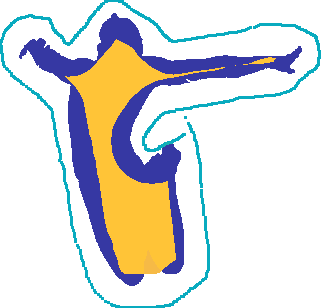
\includegraphics[width=\textwidth]{assets/img/outlineEroded.png}
    \caption{Erosion of outline}%
    \label{fig:outlineEroded}
\end{subfigure}
\hfill
\begin{subfigure}[b]{0.49\columnwidth}
    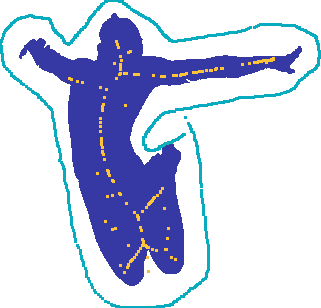
\includegraphics[width=\textwidth]{assets/img/outlineSkel.png}
    \caption{Skeleton of outline}%
    \label{fig:outlineSkel}
\end{subfigure}
\begin{subfigure}[b]{0.49\columnwidth}
    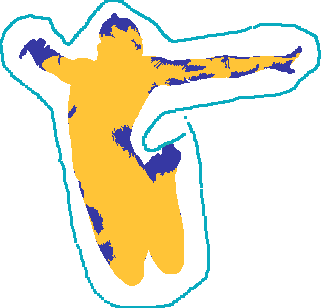
\includegraphics[width=\textwidth]{assets/img/outlineErodedSP.png}
    \caption{Erosion of outline extended with superpixels}%
    \label{fig:outlineErodedSP}
\end{subfigure}
\hfill
\begin{subfigure}[b]{0.49\columnwidth}
    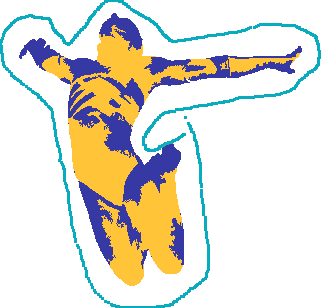
\includegraphics[width=\textwidth]{assets/img/outlineSkelSP.png}
    \caption{Skeleton of outline extended with superpixels}%
    \label{fig:outlineSkelSP}
\end{subfigure}
\caption{Different foreground inferring methods from a user outline.
The ground truth mask is in dark blue.
The user outline is in cyan.
The inferred foreground is in yellow.}%
\label{fig:foreground}
\end{figure}


\subsection{Outline erosion}%
\label{sec:erosion}


The simplest method to obtain points that are likely to be foreground
from an outline is to apply morphological erosion
of a mask representing the inside points of the outline.
We use a disk as a structuring element for the erosion,
and the only parameter of this method is the radius of the disk.


In our implementation, the disk radius is specific to each user
and computed by studying the outline performed by the user
on a reference image.
We compute the mean $m_d$ and standard deviation $s_d$ of
the distance $d$ from each outline point to the ground truth mask.
Assuming the user consistently outlines all images,
i.e.\ the mean distance of the user outline to an object
is more or less constant across all images,
a disk radius equal to $m_d + 2 \cdot s_d$ should produce an
eroded outline that is almost certainly completely foreground.


An example of this process can be visualized
on Figure~\ref{fig:outlineEroded}.
The eroded outline (yellow) is almost entirely contained
in the ground truth mask (dark blue).


\subsection{Blum medial axis algorithm}


In shape analysis and model animation, the Blum medial axis
transform~\cite{blum1978shape} is one of the most popular tools.
The Blum medial axis of a shape is composed of the centers
of the circles that are tangent to the shape in at least two points.
It is especially appropriate to compute skeletons,
composed of the medial axis points inside the shape.


\begin{figure}[ht]
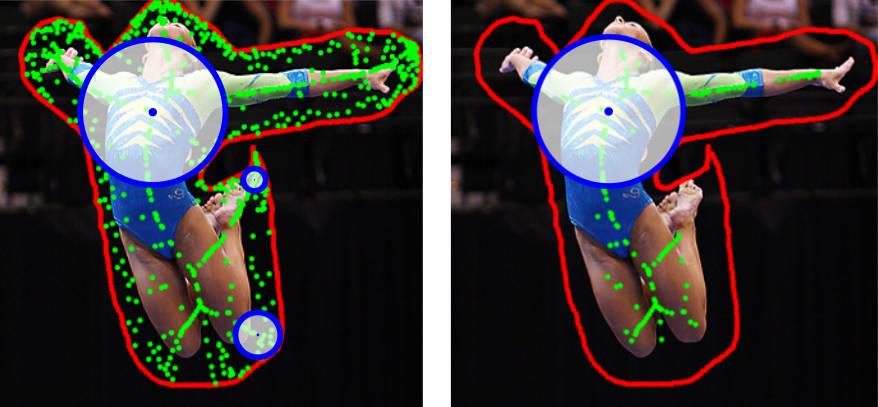
\includegraphics[width=\columnwidth]{assets/img/skeleton.jpg}
\caption{Skeleton (in green) computed using the Blum medial
axis algorithm from an outline (in red).
Few example disks are shown in blue.
In the image on the left, all disks centers (green points) are kept,
generating a very noisy skeleton.
In the image on the right the skeleton is pruned,
by filtering out centers of small disks.}%
\label{fig:skeleton}
\end{figure}


One of the problems of the medial axis algorithm is its stability
when the shape frontier is noisy.
It tends to create a high number of branches
(Figure~\ref{fig:skeleton}),
which deteriorates the simplicity of the skeleton,
and incidentally the comprehension of the shape.
In our case, this is rather an advantage.
Indeed more ramifications lead to a higher number of points
inside the shape for our foreground scribbles.
However, we need to filter the inside points,
since those close to the outline have a high probability
of being outside of the object to segment.
Radius of the inside circles of medial axis points
constitute a good filter option
because the medial axis points with the smaller radius are typically
close to the outline.
In our implementation, we choose to keep only centers
with a radius higher than half the larger radius.
Figure~\ref{fig:outlineSkel} depicts a ground truth mask in dark blue,
a user outline in cyan and the filtered medial axis points in yellow.
Most of the yellow points fall inside the ground truth mask,
thus making it a good starting point to learn the foreground model.


\subsection{Enhancing foreground with superpixels}%
\label{sec:superpixels}


These two methods, Blum medial axis and outline erosion,
allow to select foreground points that make a valuable input
to the GrabCut algorithm.
However, we add a post-processing step to (i) extend this foreground
information and (ii) filter as much false foreground points as possible.


To do so, we compute a superpixels segmentation of the image,
i.e.\ an oversegmentation that groups neighbouring pixels
with similar colorimetric properties.
We (i) extend the foreground labels from pixels
to the superpixels they belong to.
This considerably increases the surface of the foreground region.
In addition, we (ii) handle conflicting superpixels,
which contain both pixels denoted as foreground and a piece of the outline,
by removing them from the foreground mask. An example of the result
can be seen on Figure~\ref{fig:outlineErodedSP}
and Figure~\ref{fig:outlineSkelSP}.
Note that the errors arising from the first step
(between the knees in Figure~\ref{fig:outlineEroded}
and Figure~\ref{fig:outlineSkel})
have successfully been removed
in the post-processed inferred foreground mask.


We choose to use the Mean-Shift superpixels~\cite{comaniciu2002mean}
because no compacity constraint is used in their computation.
As a consequence, a superpixel can cover a large area
(especially in the case of similar background regions,
such as an homogeneous sky) and will more likely correct
wrongly inferred foreground points.


%%%%%%%%%%%%%%%%%%%%%%%%%%%%%%%%%%%%%%%%%%%%%%%%%%%%%%%%%%%%%%%%%%%%%%%


\section{Experiments}%
\label{sec:experiment}


In this section we describe the setup of our experiments
and analyze the outcome of the study.


\subsection{Experimental setup}


\textbf{Interactions}
Since the subject of the study is interactive segmentation on touch devices,
we choose to compare only three annotations:
outlines, scribbles, and bounding boxes.
We do not include polygon drawing since
it is clearly not adapted to a touch device.
Indeed, fingers are too big to precisely touch the boundary of an object,
they would hide the area where the user should try to place the vertex on.


The interfaces are kept as simple as possible.
The user is shown an image and has to provide a valid input
to be allowed to move on to the next image.


\begin{figure}[ht]
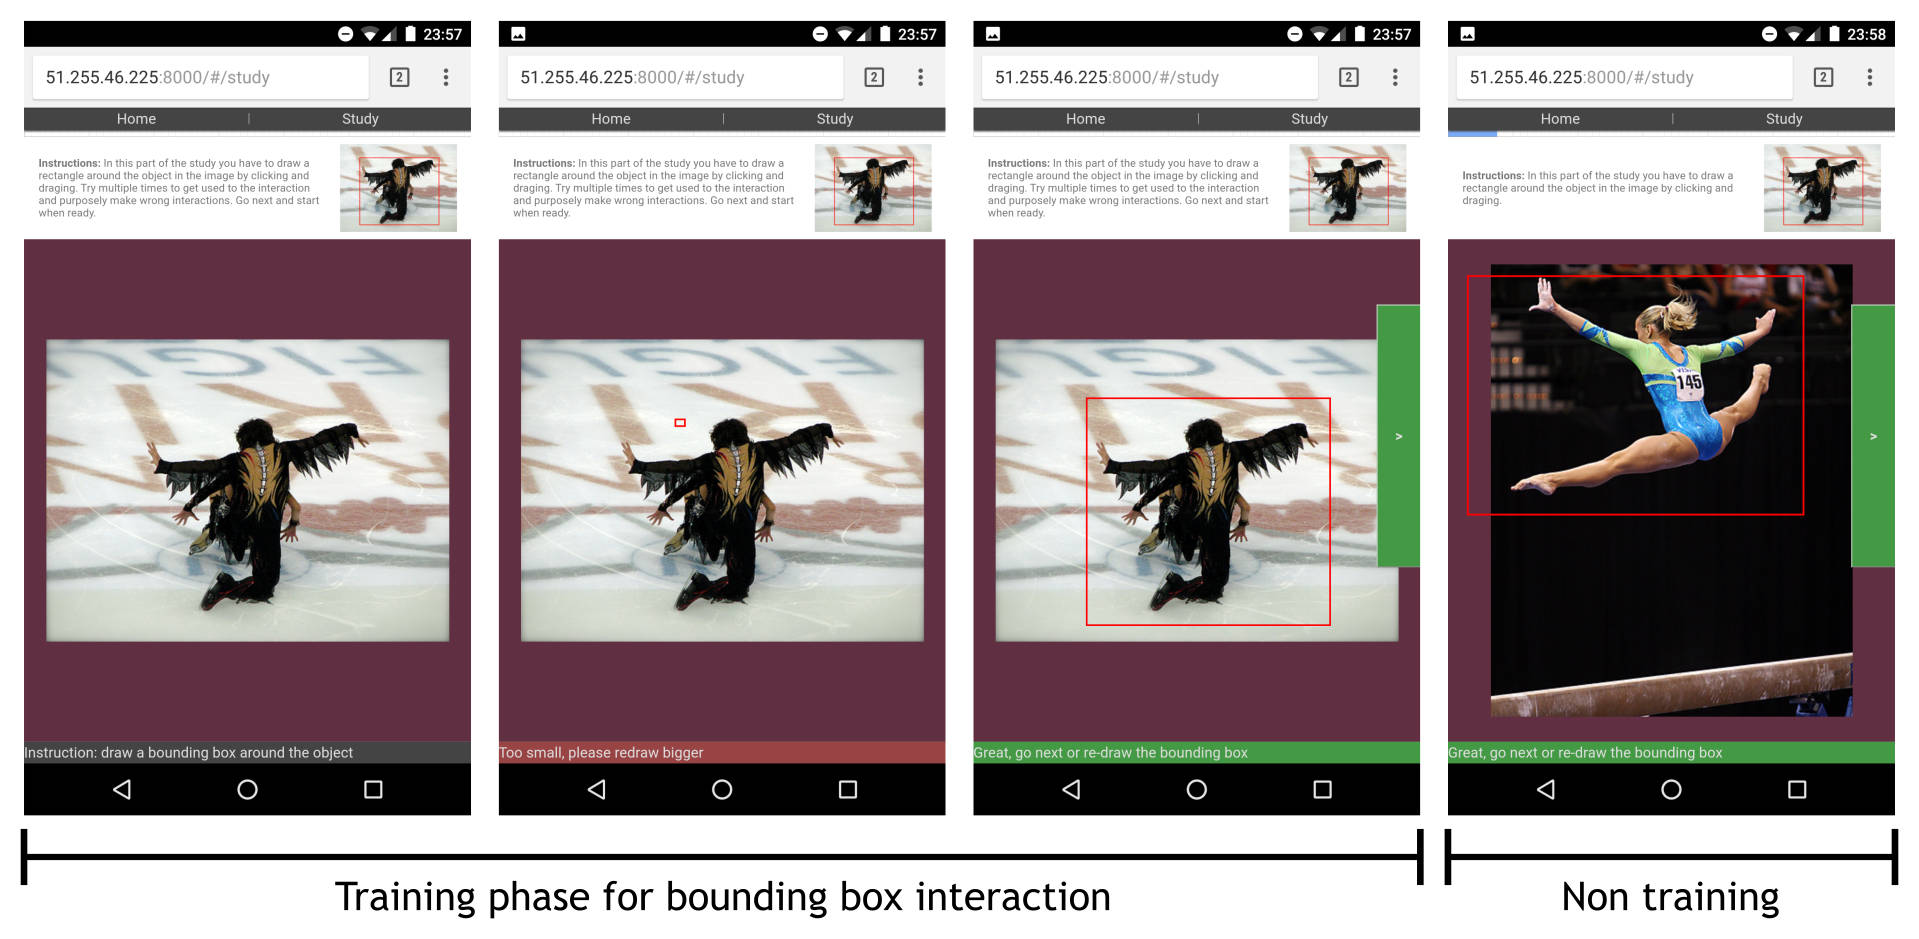
\includegraphics[width=\columnwidth]{assets/img/app_rect.jpg}
\caption{Several screenshots of the bounding box interface
during training (left) and study (right) phases.
Some minimal input validation is performed, such as checking
that the surface of the annotation is above a minimal threshold.
If not, a message with a red banner is displayed at the bottom
of the screen as in the second image above.}%
\label{fig:rectangle}
\end{figure}


The bounding box interface allows the user to draw a rectangle
over the image using a touch and drag interaction (Figure~\ref{fig:rectangle}).
If the user is not satisfied with their previous attempt,
they can start over, which will replace the former rectangle with a new one.
The user can only move on to the next image when the current rectangle
is of sufficient size (we discard rectangles
that are too small to avoid common mistouch issues).


\begin{figure}[ht]
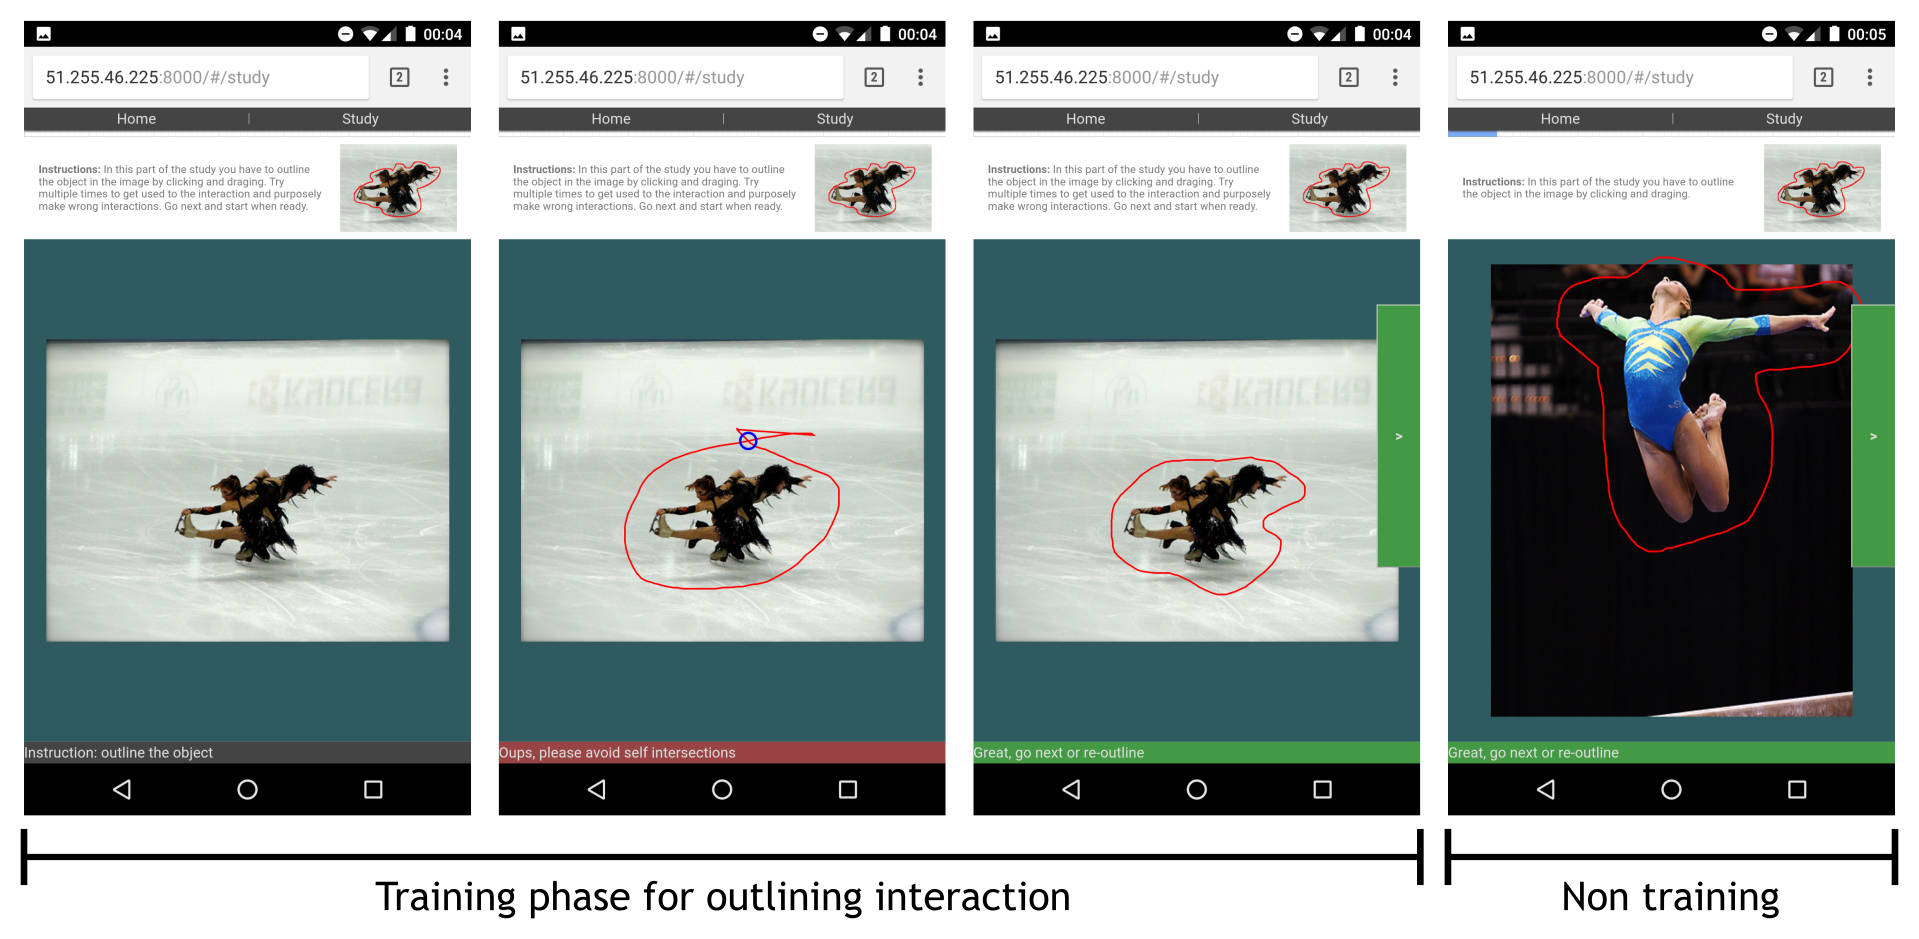
\includegraphics[width=\columnwidth]{assets/img/app_outline.jpg}
\caption{Several screenshots of the outlining interface
during training (left), and study (right) phases.}%
\label{fig:outline}
\end{figure}


The outlining interface is very similar to the bounding box interface.
The user can draw the outline using a touch and drag interaction;
the system automatically draws the closing segment between
the ending and starting points when the user releases their finger.
The user can also start over if not satisfied with the current outline.
The system allows the user to move on to the next image
if the outline is of sufficient area.
In addition, for the training image only,
the system checks the absence of loops in the outline path
(Figure~\ref{fig:outline}), for they may reveal incorrect usage.
This loop detection feature is deactivated for the other images
to limit its impact on the interaction and user frustration.


\begin{figure}[ht]
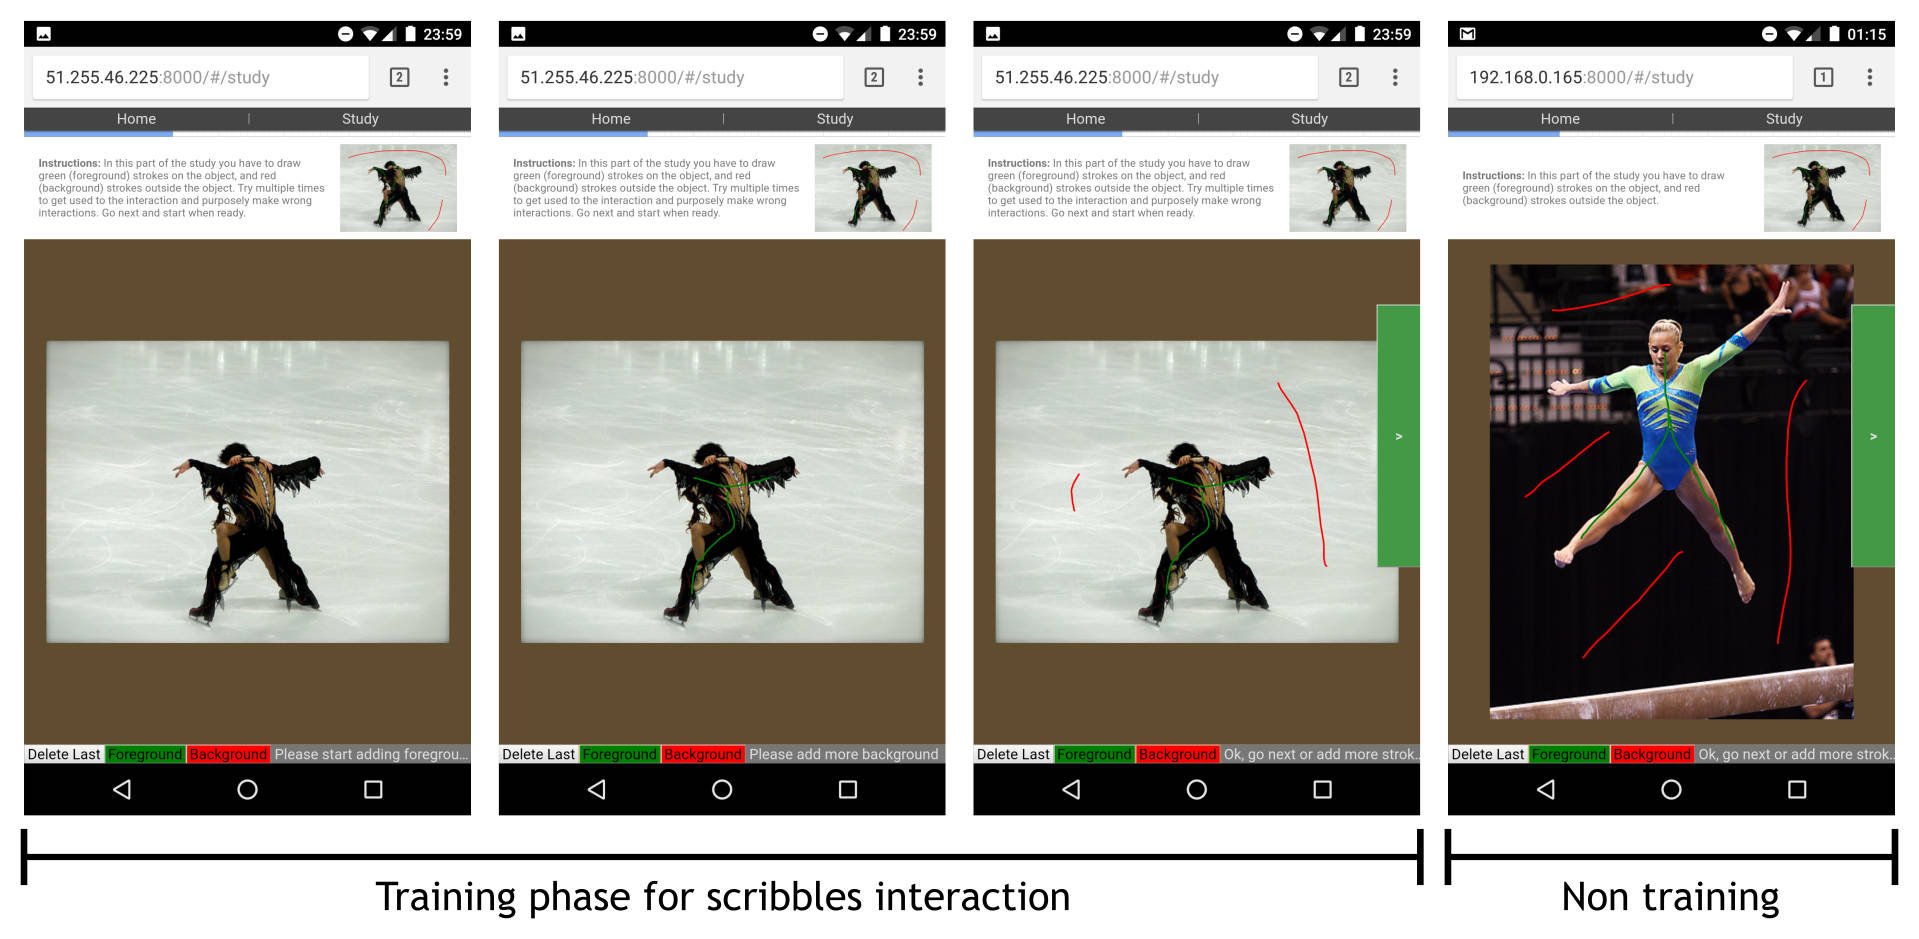
\includegraphics[width=\columnwidth]{assets/img/app_scribbles.jpg}
\caption{Several screenshots of the scribbling interface
during training (left), and study (right) phases.}%
\label{fig:scribbles}
\end{figure}


The scribbling interface displays three buttons:
one to select the foreground scribbles, which are drawn in green,
one to select the background scribbles, which are drawn in red,
and one to remove the last drawn scribble.
Users are required to provide at least a minimum scribble length
to be allowed to move on to the next image.


\textbf{Device and software}
We use a regular 8'' android tablet,
for which the buttons appear large enough to be easily clickable.
The user study is conducted on a Web application in the Chrome browser for android.
The code for this study (Web client and server),
as well as the results presented here are all available online
(github.com/mpizenberg/otis).


\textbf{Images}
We select 36 images from the iCoseg dataset~\cite{batra_icoseg:_2010},
which we divide into 3 groups of 12 images.
We want the segmentation results to be comparable between
different interactions, but since each user tests the three interfaces,
we do not want the same images for every phase of the study.
This would risk biasing the results since
users might get annoyed of annotating three times the same images,
affecting the quality of their annotations.
The iCoseg dataset provides multiple images depicting the same object
in different situations so we use similar images in the 3 groups.
Examples of these images can be seen on Figure~\ref{fig:icoseg}.


\begin{figure}[ht]
\centering
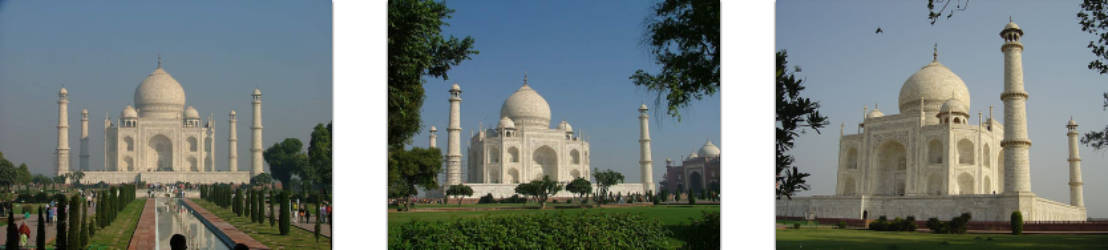
\includegraphics[width=\columnwidth]{assets/img/taj_mahal.jpg}
\vfill\vspace{0.5em}\vfill
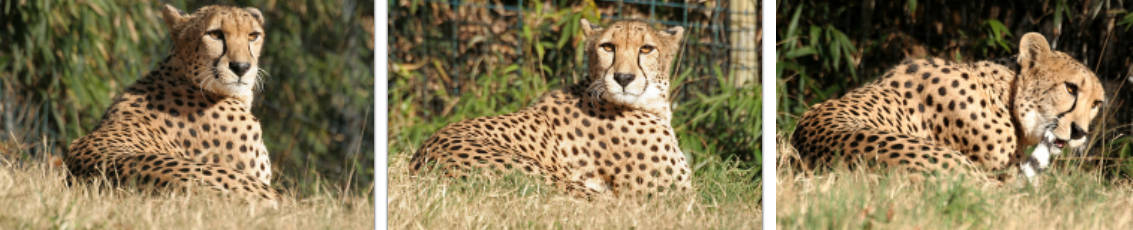
\includegraphics[width=\columnwidth]{assets/img/cheetah.jpg}
\caption{Some images from the iCoseg dataset.}%
\label{fig:icoseg}
\end{figure}


\textbf{Methodology}
The protocol of the study is as follows.


The users are not explained the concept of segmentation,
we tell them that we require annotations on images,
and that we wish to compare three interactions to provide those annotations.


The study is composed of three steps, one step per interaction.
For each step, the evaluator first explains the user how
the interaction works, and demonstrates it on a training image.
The evaluator demonstrates good and bad examples of interactions.
Then the user tests the interaction on the same training image.
The evaluator can correct the user and criticize or validate
the users interactions.
Once the user understands the tool,
the eleven other images are proposed for interaction,
without any help or guidance from the evaluator.
Finally, at the end of each step,
the user answers two questions about the interaction.
In order to limit bias, the order of the interactions is randomized,
as well as the order of appearance of each image during each step.


Among the eleven images annotated by the user,
one is considered the reference.
It is introduced to (i) check whether the user is performing the task
correctly (this is particularly useful in a crowdsourcing context),
and (ii) to learn the radius of the erosion disk for this specific user
(see Section~\ref{sec:erosion}).


The following two questions are asked at the end of each step of the study.
\vspace{-1em}
\begin{itemize}
\setlength\itemsep{-0.5em}
\item Overall, I am satisfied with the ease of
 completing the tasks in this scenario.
\item Overall, I am satisfied with the amount of time
 it took to complete the tasks in this scenario.
\end{itemize}
Users can answer on a scale
from 1 (strongly agree) to 7 (strongly disagree).
We choose to ask only these two questions since we are not trying
to assess the usability of a whole system, but only of an interaction.
A standard usability questionnaire,
such as SUS (used in~\cite{korinke_exploring_2015}),
was not really adapted to our use case and instead
we extracted these two questions from a popular post-task questionnaire
(ASQ, After Scenario Questionnaire).


Finally at the end of the study, we ask users to rank
the three interactions in their order of preference
(see ``Rank'' in Table~\ref{tab:questionnaire}).


\textbf{Participants}
Twenty users (10 Male, 10 Female) participated to this study,
with ages ranging from 25 to 55 years old.
Most users have no experience in image segmentation,
some of them are familiar with the concept.


\subsection{Usability metrics}


Among the criteria stated by Nielsen~\cite{nielsen1994usability}
as defining the usability of a system,
we evaluate efficiency, errors, and user satisfaction.
Efficiency designates the swiftness with which users are able
to complete the tasks once they learn how to interact with the system.
We evaluate this criterion both subjectively,
by asking users about their perception of the time
they spent on the task (table~\ref{tab:questionnaire}),
and objectively by measuring the time it takes to complete their
interactions on each image (Figure~\ref{fig:timeinteraction}).
User satisfaction is measured through our questionnaire,
both by the question on the perceived task easiness
and the interaction ranking.
Finally, errors are measured by counting the number of times
users repeat interactions.
We record how many times bounding boxes and outlines are re-drawn,
and the number of clicks on the \textit{Undo last scribble} button
for the scribbling interaction
(Figure~\ref{fig:errorinteraction}).


\begin{table}[ht]
\centering
\begin{tabular}{lrrr}
Method & Bounding box & Outline & Scribble \\ \midrule
Ease & 2.1 $\pm$ 0.62 & 2.65 $\pm$ 0.74 & 2.1 $\pm$ 0.61 \\
Time & 2.35 $\pm$ 0.69 & 2.5 $\pm$ 0.67 & 2.6 $\pm$ 0.70 \\
Rank & 1.95 $\pm$ 0.43 & 1.90 $\pm$ 0.32 & 2.15 $\pm$ 0.37 \\
\end{tabular}
\caption{Results of the questionnaire with a 95\% confidence interval.}%
\label{tab:questionnaire}
\end{table}


\begin{figure}[ht]
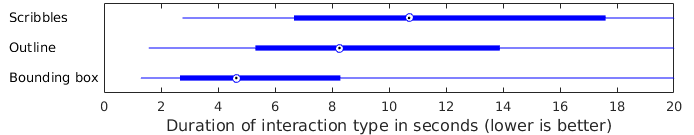
\includegraphics[width=\columnwidth]{assets/plot/interactions_durations.png}
\caption{Duration of interactions on all images and all users.
The dots are the median durations, and the thick blue line delimits
the first and third quartiles.}%
\label{fig:timeinteraction}
\end{figure}


\begin{figure}[ht]
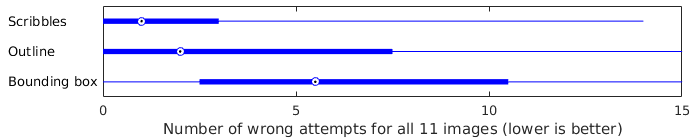
\includegraphics[width=\columnwidth]{assets/plot/interactions_errors_per_user.png}
\caption{Number of errors per interaction and per user on all images.
The dots are the median number of errors,
and the thick blue line delimits the first and third quartiles.}%
\label{fig:errorinteraction}
\end{figure}


Overall, the questionnaire results can not allow us to conclude
on the superiority of one interaction method over the others.
Although slightly in favor of the bounding box interaction,
the perceived ease and time are not statistically better
for any of the three interactions.
However, the results are all between 2 and 3 (on a scale from 1 to 7),
which means users were mostly satisfied with all three interactions.
We can note that the time perception results
(table~\ref{tab:questionnaire}) are correlated with the
objective duration of interaction (Figure~\ref{fig:timeinteraction}),
measured during the experiments.
The bounding box is the quickest interaction,
while the scribbles suffer from the time needed to switch between
foreground and background scribbling.


Surprisingly, the outline ranks first in the users preference
(although not significantly), ahead of the bounding box interaction.
The reason of this observation, as explained by many of the participants
during the experiment, is due to the frustration
that can arise when trying to draw a bounding box
around a non-convex object.
Users trying to draw the bounding box close
to the object boundary often need several attempts,
because of the difficulty to position the first bounding box corner.
This issue is visible on Figure~\ref{fig:errorinteraction},
which shows the high number of errors for bounding boxes.
Errors occurring with the outline interaction are mostly due
to high speed interactions,
or due to masking the object with their hand during the interaction
for users less familiar with touch devices.


\subsection{Interaction informativeness}


We define the background area of user inputs as follows.
For a bounding box (resp.\ outline), the background area is composed
of all pixels outside of the bounding box (resp.\ outline).
For scribbles, the background area is the union of the superpixels
annotated as background (containing part of a background scribble).


\begin{figure}[ht]
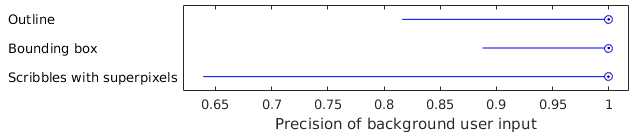
\includegraphics[width=\columnwidth]{assets/plot/precision_bg_all.png}
\caption{Precision of background user input.}%
\label{fig:precision_bg}
\end{figure}


\begin{figure}[ht]
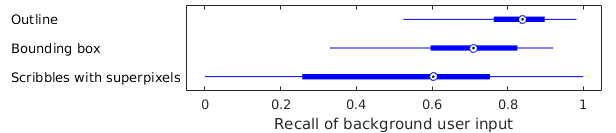
\includegraphics[width=\columnwidth]{assets/plot/recall_bg_all.png}
\caption{Recall of background user input.}%
\label{fig:recall_bg}
\end{figure}


Looking at the precision of background user inputs
(Figure~\ref{fig:precision_bg}) we see that more than
75\% of user annotations are perfect (a precision score of 1).
This means that 75\% of user inputs do not intersect at all
the object of interest.
We can conclude that users understand well the tasks they are given.


In order to estimate the informativeness of an interaction,
we also measure the recall index (Figure~\ref{fig:recall_bg}).
It indicates the percentage area of all background
that is annotated by an interaction.
With no surprise, outlining is the more informative
since it is often very close to the boundary of the object
(Figure~\ref{fig:complexoutlines}) and thus,
the outside of the outline covers most of the image background.
Background (red) scribbles are the least informative here since only
superpixels that are scribbled over count as background information.


Except for the foreground (green) scribble interaction,
we do not have raw foreground annotations.
We thus define the foreground input area as the inferred foreground
(through erosion or medial axis computation,
extended by superpixels as explained previously).


\begin{figure}[ht]
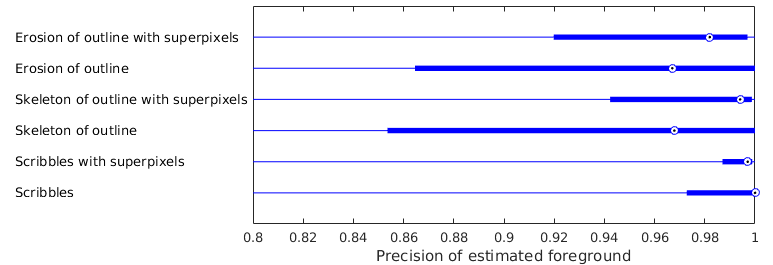
\includegraphics[width=\columnwidth]{assets/plot/precision_fg_all.png}
\caption{Precision of foreground user input.}%
\label{fig:precision_fg}
\end{figure}


\begin{figure}[ht]
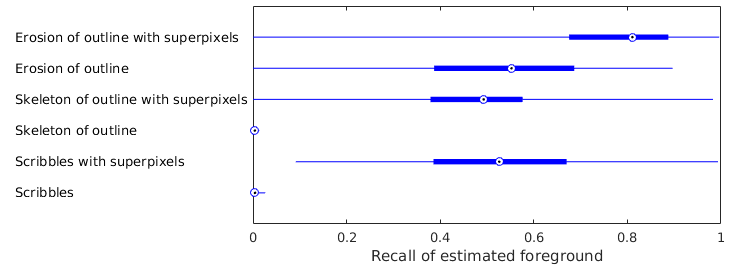
\includegraphics[width=\columnwidth]{assets/plot/recall_fg_all.png}
\caption{Recall of foreground user input.}%
\label{fig:recall_fg}
\end{figure}


The precision of foreground area is given in
Figure~\ref{fig:precision_fg}, relatively to the ground truth masks.
We can observe that more than 75\% of foreground (green)
scribble inputs are over the 0.97 index.
This means that the task of scribbling inside the objects
is globally well performed but still slightly harder
than background (red) scribbles.
It is explained by the fact that objects can have thin shapes
and thus not precisely locatable under the finger
during the touch interaction.


Using the superpixels extension of the scribbles,
we observe that the smart background correction mentioned
in Section~\ref{sec:superpixels},
enhances the 75\% index to a precision of 0.99.
With the two foreground inference techniques (erosion and skeleton),
the improvement provided by the superpixels extension is obvious.


The recall of foreground area (Figure~\ref{fig:recall_fg})
provided by these interactions, extended through superpixels is
also coherent with what we observe in Figure~\ref{fig:foreground}.
Skeleton and scribbles recall values are almost 0 since they are of
dimension 0/1 (points/lines) for a measure of surfaces (dimension 2).
Erosion provides the most foreground information,
but has the lower precision rate (Figure~\ref{fig:recall_fg}).
We will show in the next section that this trade-off is worth exploring.


\subsection{Segmentation quality}


We compute the resulting segmentation of images using five different methods.
As a reference method, the mean Jaccard index obtained with foreground
and background scribbles is 0.79 (Table~\ref{tab:jaccard}).
When using bounding boxes, that provide a more complete
background model input for the GrabCut algorithm,
the mean Jaccard index increases to 0.82.
As expected, it increases even more when using outlining interaction inputs,
providing richer inferred initial foreground models to the GrabCut algorithm.
The higher scores (0.88 and 0.89) are respectively obtained when
using the erosion and skeleton processing of the outline.
The best performance is achieved using the skeleton processing,
which tends to show that for the results presented in the previous section,
the precision of the foreground user input is more relevant than its recall.


\begin{table}[ht]
\centering
\begin{tabular}{cccccc}
Method & Scrib. & B. Box & Outl. & Outl. + er. & Outl. + BMA \\ \midrule
Mean Jaccard & 0.79 & 0.82 & 0.86 & 0.88 & 0.89 \\
\end{tabular}
\caption{Mean Jaccard index obtained on all images
for all users for each interaction.}%
\label{tab:jaccard}
\end{table}


\begin{figure}[ht]
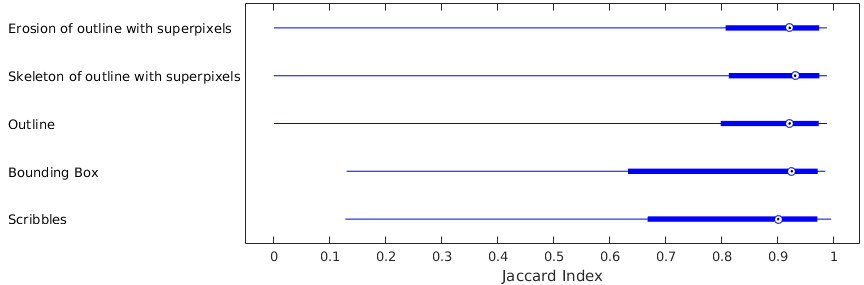
\includegraphics[width=\columnwidth]{assets/plot/jaccard.png}
\caption{Jaccard index obtained on all images for all users
for each interaction type.}%
\label{fig:jaccard}
\end{figure}


\begin{figure}[ht]
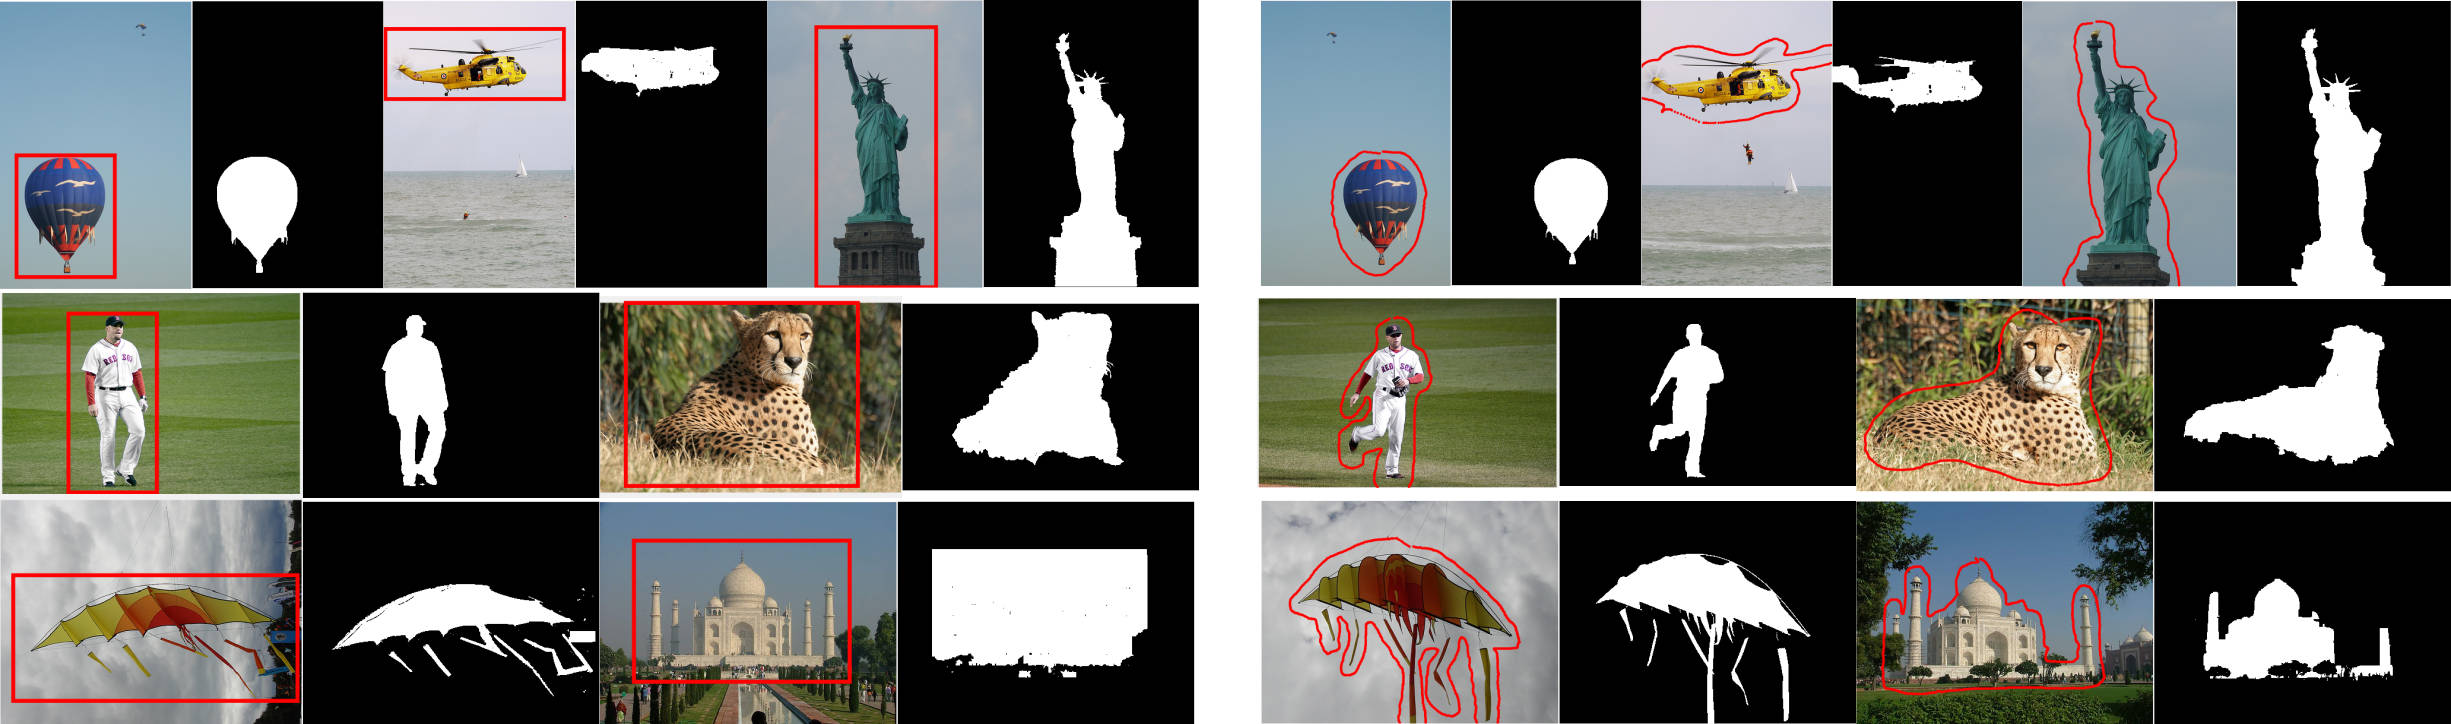
\includegraphics[width=\textwidth]{assets/img/results.jpg}
\caption{Segmentation results for bounding box
and outlining interactions from a user.}%
\label{fig:results}
\end{figure}


Perhaps more importantly, the outlining interaction enables reaching
consistently higher Jaccard index than the other techniques.
In Figure~\ref{fig:jaccard}, we observe that the first quartile is
always higher than 0.8 with variants of the outlining interaction.
Some final segmentation results are visible in Figure~\ref{fig:results}
and show the clear improvement brought by an outline over a bounding box.


\subsection{Discussion}


All the results we obtained confirm the good properties
of the outlining interaction in the perspective of being used
in a segmentation crowdsourcing campaign.


First, it is a very straightforward interaction.
One of the users explained it in these terms:
\textit{outlining is easier since you do not need to think,
just trace the object.
Bounding boxes are tougher, particularly in determining a correct size,
and scribbles is too much thinking and a bit more time consuming.}
Another user said: \textit{It's actually more fun to draw around object
and would seem to me less tiring than the other methods}.
The usability criterion points out that outlining might be slightly less
usable than drawing a bounding box or scribbling,
but remains a very usable interaction.


Another interesting property of the outlining interaction
is the speed at which it can be performed.
Figure~\ref{fig:timeinteraction} shows that most of the outlines
were produced in less than 10 seconds,
which is very reasonable considering some of the images we chose have
complex shapes (Figure~\ref{fig:complexoutlines}).


\begin{figure}[ht]
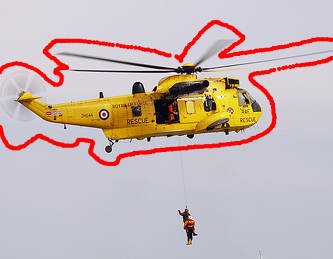
\includegraphics[width=0.31\columnwidth]{assets/img/helicopter_02_annot.jpg}\hfill
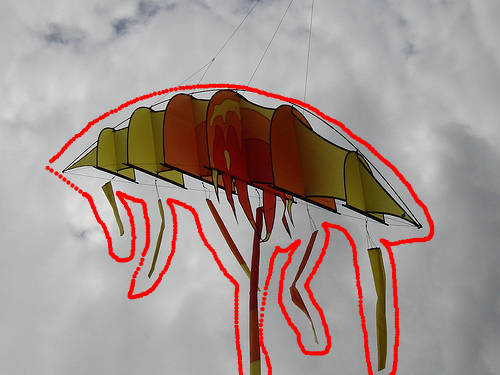
\includegraphics[width=0.32\columnwidth]{assets/img/kite_02_annot.jpg}\hfill
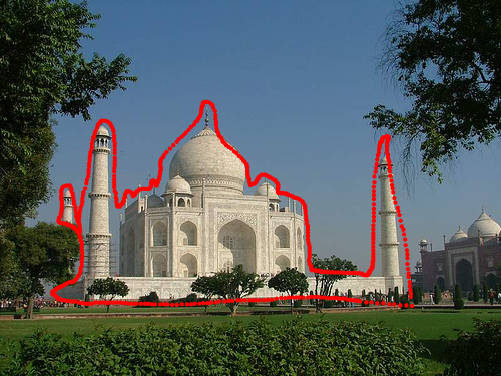
\includegraphics[width=0.32\columnwidth]{assets/img/taj_mahal_02_annot.jpg}
\caption{Outlines drawn by the third user on three images with complex shapes.}%
\label{fig:complexoutlines}
\end{figure}


The quantity of information brought by outlines is also very good,
as discussed in the previous section,
especially when balanced with the interaction usability.
This information is of course less complete than a polygon drawn
on the boundary of the object (such as in LabelMe),
but can be augmented using computer vision techniques (Blum medial axis,
superpixels, GrabCut, etc.) and lead to very good segmentation masks.
The average Jaccard index of 0.89 obtained with the outlines
is particularly impressive considering there was no interactive refinement step,
and it was performed in less than 10 seconds in average
(see for example the comparison with Jaccard index vs.\
time curves described in~\cite{carlier_clickncut:_2014}).


\section{Conclusion}


In this chapter, we evaluated the outlining interaction
on touch devices for interactive segmentation.
We found that outlining is a simple and natural interaction, allowing
to quickly obtain accurate information on the location of an object.
This information can be augmented with foreground inference,
and then used to compute a segmentation mask.
The segmentation masks obtained with this method reach an average
Jaccard index of 0.89, which is a very good result
considering the interaction does not require any knowledge
on image processing or computer vision from the user.


Thanks to all these good properties (simplicity, swiftness, accuracy),
outlining appears to be an interesting avenue to explore for the gathering
of large datasets of image segmentation masks.
Those datasets are crucial to bring automatic image segmentation algorithms,
today mostly based on deep learning techniques, to a new level of effectiveness.
It is our intention to pursue this goal so
we will next introduce an annotation Web application
built to easily start a crowdsourcing campaign on Amazon Mechanical Turk.
